\section{Model}\label{sec:Model}
Das Model repräsentiert die zugrunde liegende logische Struktur von Daten in der Tableau-Anwendung. Das Klassendiagramm des Models ist in Abbildung \ref{fig:KlassendiagrammModel} gezeigt.

\begin{figure}[!h] \centering

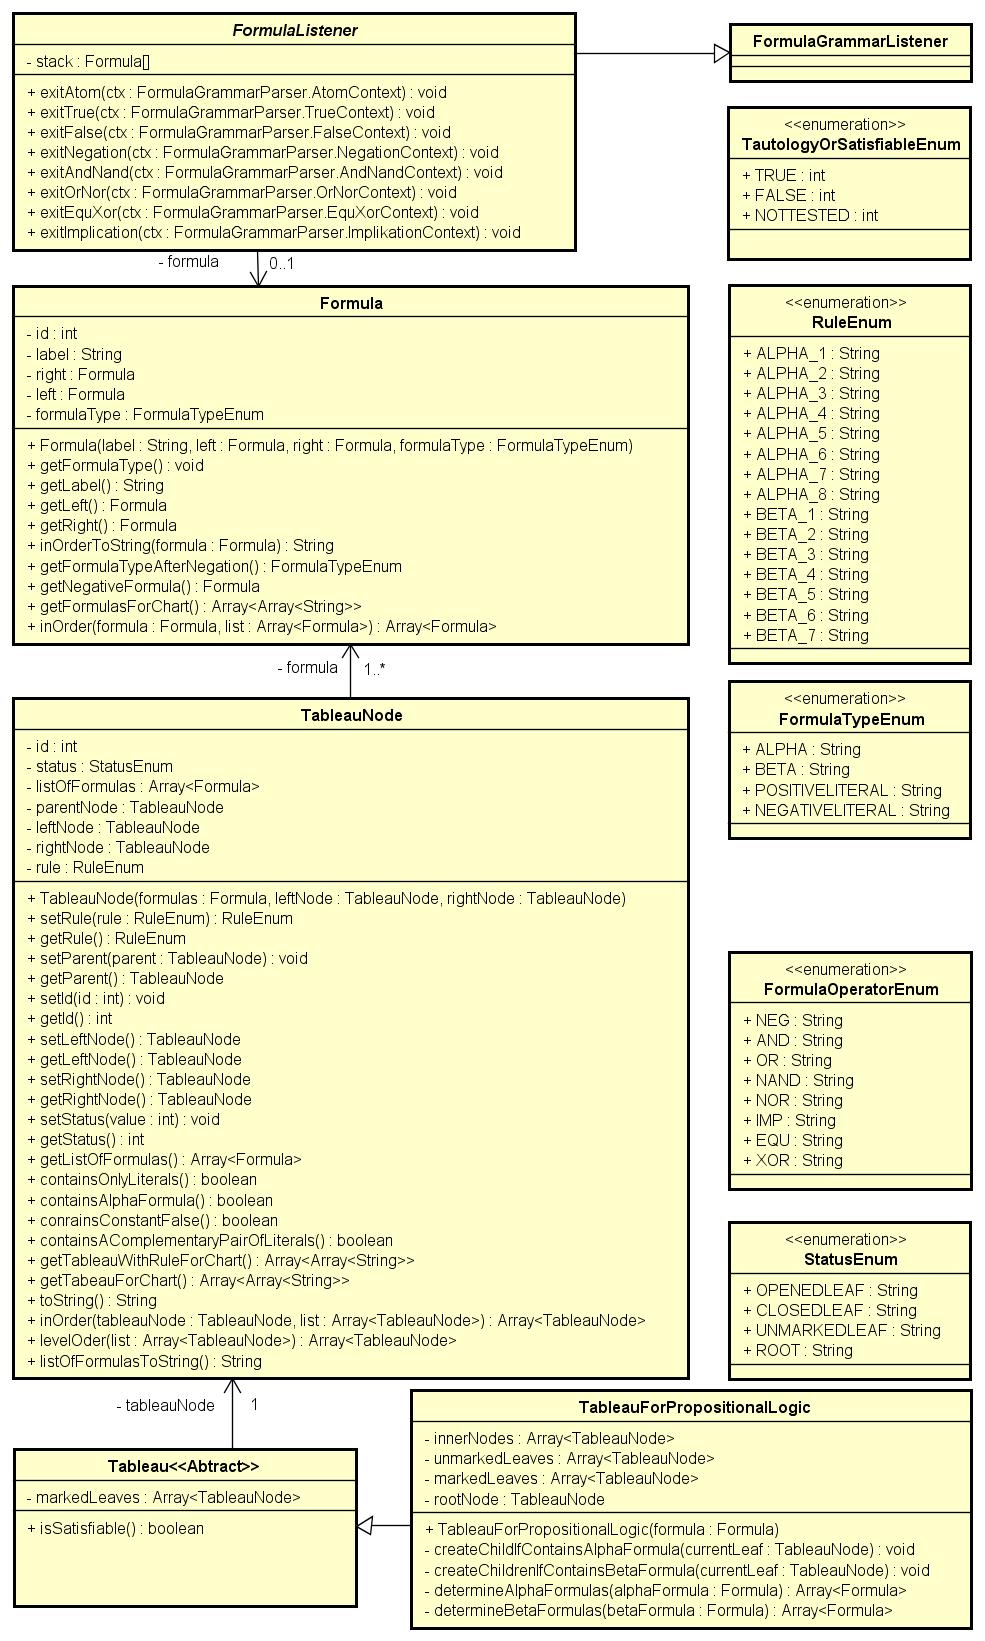
\includegraphics[width=0.9\textwidth]{ClassDiagramModel}
\caption[KlassendiagrammModel]{Klassendiagramm(Model)}\label{fig:KlassendiagrammModel}

\end{figure}

\subsection{Formula}
Aus der Definition \ref{Definition 2.2} ist es möglich, dass jede Formel als ein Binärbaum dargestellt werden kann. Der Baum besteht aus Knoten (\textit{Formula}). Jeder Knoten hat einen linken Teilbaum (\textit{left}), einen rechten Teilbaum (\textit{right}), die auch Knoten sind und einen Inhalt (\textit{label}), welcher eine Aussagenvariable oder ein Junktor (Definition \ref{Definition 2.1}) ist \cite{Krohn}. Die Junktoren werden in der Enumeration \textit{FormulaOperatorEnum} definiert.
\begin{lstlisting}[language=JavaScript, caption= FormulaOperatorEnum, basicstyle=\scriptsize]
const FormulaOperatorEnum = Object.freeze({
    NEG: "\u00AC",
    AND: "\u2227",
    OR:  "\u2228",
    NAND:"\u2191",
    NOR: "\u2193",
    IMP: "\u2192",
    EQU: "\u2194",
    XOR: "\u2295"
});
exports.FormulaOperatorEnum = FormulaOperatorEnum;
\end{lstlisting}

Weiterhin kann eine Formel ein Literal (Definition \ref{Definition 2.57}), $\alpha$- oder $\beta$-Formel (Tabelle \ref{Abb. 2.8}) sein. Diese Formeltypen werden in der Enumeration \textit{FormulaTypeEnum} definiert und werden in dem Attribut \textit{formulaType} der Klasse \textit{Formula} gespeichert. Aus der Bemerkung \ref{FormelAlsString} kann der Ausdruck als String von einer Formel durch eine In-order-Baumtraversierung erhalten werden. Um diesen Ausdruck korrekt abzubilden (z.B. $\neg$q nicht q$\neg$), hat die Formel, die mit einer $\neg$ (oder \textit{FormulaOperatorEnum.NEG}) gekennzeichnet wird, immer nur ein rechtes Kind, d.h \textit{left} ist ``\textit{Null}''. Wenn eine Formel ein Blatt ist, sind beide (\textit{left} und \textit{right}) auch ``\textit{Null}''. Damit die Formel mittels Google Charts visualisiert werden kann (Unterabschnitt \ref{Organigramm}), muss jeder Knoten eine eindeutige Kennzeichnung (\textit{id}) haben.

\begin{lstlisting}[language=JavaScript, caption= FormulaTypeEnum, basicstyle=\scriptsize]
const FormulaTypeEnum = Object.freeze({
    ALPHA: "ALPHA",
    BETA: "BETA",
    NEGATIVLITERAL: "NEGATIVLITERAL",
    POSITIVLITERAL: "POSITIVLITERAL",
    TRUE: "TRUE",
    FALSE: "FALSE"
});
\end{lstlisting}

Um die Tautologie einer Formel zu überprüfen, benötigt es die Negation der Formel. Daher bietet Klasse \textit{Formula} die Methode \textit{getNegativeFormula()}. Nach der Negation wird der Formeltyp geändert, deshalb wird die Methode \textit{getFormulaTypeAfterNegation()} implementiert, um den neuen Formeltyp zu bestimmen.

\begin{lstlisting}[language=JavaScript, caption= getNegativeFormula() und getFormulaTypeAfterNegation() (Klasse Formula) , basicstyle=\scriptsize]
Formula.prototype.getFormulaTypeAfterNegation = function () {
    var formulaType;
    if (this.getFormulaType() == FormulaTypeEnum.TRUE) {
        formulaType = FormulaTypeEnum.FALSE;
    } else if (this.getFormulaType() == FormulaTypeEnum.FALSE) {
        formulaType = FormulaTypeEnum.TRUE;
    } else if (this.getFormulaType() == FormulaTypEnum.POSITIVLITERAL) {
        formulaType = FormulaTypeEnum.NEGATIVLITERAL;
    } else if (this.getLabel() == FormulaOperatorEnum.NEG) {
        formulaType = FormulaTypeEnum.ALPHA;
    } else if (this.getFormulaType() == FormulaTypeEnum.ALPHA) {
        formulaType = FormulaTypeEnum.BETA;
    } else {
        formulaType = FormulaTypeEnum.ALPHA;
    }
    return formulaType;
};

Formula.prototype.getNegativeFormula = function () {
    var negationFormulaType = this.getFormulaTypeAfterNegation();
    var negationFormula = new Formula(FormulaOperatorEnum.NEG, null, this, negationFormulaType);
    return negationFormula;
};
\end{lstlisting}

Außerdem bietet Klasse \textit{Formula} die folgenden Methoden:
\begin{itemize}
\item	\textit{inOrder()}: Rekusive Methode, die eine Liste der Knoten durch In-Order-Baumtraversierung zurück gibt. 
\item	\textit{inOrderToString()}: Gibt Ausdruck als String von der Formel zurück.
\item	\textit{getFormulasForChart()}: Erzeugt ``Google Charts DataTable'' um die Formel zu visualisieren. Die DataTable ist ein zweidimensionales Array. Jedes Element des Arrays beschreibt einen Knoten mit \textit{id} des Knotens und der \textit{id} des übergeordneten Knotens. Diese Ids werden nicht angezeigt. Im Diagramm wird nur das \textit{label} des Knotens angezeigt. Alle Elemente des Arrays werden durch In-Order-Baumtraversierung sortiert.
\end{itemize}

\begin{lstlisting}[language=JavaScript, caption= getFormulasForChart()(Klasse Formula), basicstyle=\scriptsize]
Formula.prototype.getFormulasForChart = function () {
    var ret = [];
    var list = [];
    var arr = [];
    list = this.inOrder(this, list);
    for (var i = 0; i < list.length; i++) {
        list[i].id = i;
    }
    ret.push([{v: this.id.toString(), f: this.label}, ""]);
    for (var i = 0; i < list.length; i++) {
        if (list[i].left != null) {
            arr = [{v: list[i].left.id.toString(), f: list[i].left.label}, list[i].id.toString()];
            ret.push(arr);
        }
        if (list[i].right != null) {
            arr = [{v: list[i].right.id.toString(), f: list[i].right.label}, list[i].id.toString()];
            ret.push(arr);
        }
    }
    return ret;

};
\end{lstlisting}

\subsection{FormulaListener}
Mit ANTLR kann man den Parse-tree mit einem benutzerdefinierten Listener oder einem benutzerdefinierten Visitor besuchen.
Beide Implementierungen geben dasselbe Ergebnis aus. Die Visitor-Implementierung hat aber einen Vorteil, da die Visitor-Methoden einen Wert zurück geben und keine Werte in Feldern gespeichert werden müssen. Dagegen wird die Listener-Implementierung in dieser Arbeit gewählt, da diese im JavaScript bekannter ist und es viele Beispiele im Internet sowie auf der offiziellen Seite \url{https://github.com/antlr/antlr4/blob/master/doc/javascript-target.md} gibt.

\textit{FormulaListener} definiert einen benutzerdefinierten Listener um die Syntaxbaum zu besuchen. Diese Klasse erweitert die Klasse \textit{FormulaGrammarListener}, eine Klasse welche die ANTLR-Runtime automatisch generiert hat.

\begin{lstlisting}[language=JavaScript, caption= FormulaListener Konstruktor, basicstyle=\scriptsize]
 var FormulaListener = function () {
    FormulaGrammarListener.call(this);
};

FormulaListener.prototype = Object.create(FormulaGrammarListener.prototype);
\end{lstlisting}


\textit{FormulaGrammarListener} definiert alle Methoden, die die Klasse \textit{ParseTreeWalker} von der ANTLR-Runtime auslösen kann, wenn sie den Parse-tree durchläuft. Um die Eingabeformel zu analysieren muss man auf acht Ereignisse reagieren, indem man acht Methoden überschreibt: Wenn der Walker eine Aussagenvariable, einen Junktor oder eine Konstante verlässt. Hier sind die relevanten Methoden von der generierten Klassen \textit{FormulaGrammarListener}: 

\begin{lstlisting}[language=JavaScript, caption= FormulaGrammarListener, basicstyle=\scriptsize]
function FormulaGrammarListener() {
	antlr4.tree.ParseTreeListener.call(this);
	return this;
}

FormulaGrammarListener.prototype = Object.create(antlr4.tree.ParseTreeListener.prototype);

FormulaGrammarListener.prototype.constructor = FormulaGrammarListener;
// Exit a parse tree produced by FormulaGrammarParser#Atom.
FormulaGrammarListener.prototype.exitAtom = function(ctx) {};

// Exit a parse tree produced by FormulaGrammarParser#True.
FormulaGrammarListener.prototype.exitTrue = function(ctx) {};

// Exit a parse tree produced by FormulaGrammarParser#False.
FormulaGrammarListener.prototype.exitFalse = function(ctx) {};

// Enter a parse tree produced by FormulaGrammarParser#Negation.
FormulaGrammarListener.prototype.enterNegation = function(ctx) {};

// Exit a parse tree produced by FormulaGrammarParser#AndNand.
FormulaGrammarListener.prototype.exitAndNand = function(ctx) {};

// Exit a parse tree produced by FormulaGrammarParser#OrNor.
FormulaGrammarListener.prototype.exitOrNor = function(ctx) {};

// Exit a parse tree produced by FormulaGrammarParser#EquXor.
FormulaGrammarListener.prototype.exitEquXor = function(ctx) {};

// Exit a parse tree produced by FormulaGrammarParser#Implication.
FormulaGrammarListener.prototype.exitImplikation = function(ctx) {};

\end{lstlisting}

Da Listener-Methoden keinen Wert zurück geben, muss \textit{FormulaListener} ein Array \textit{stack} um die besuchende Formeln zu speichern, haben. Weiterhin hat \textit{FormulaListener} folgende überschriebenen Methoden. Jede Methode hat ein Argument \textit{ctx}. Das Argument ctx ist eine Instanz eines spezifischen Klassenkontextes für den Knoten, den Walker verlässt.

\begin{itemize}

\item	\textit{exitAtom()}: Diese Methode fügt eine neue Aussagenvariable im \textit{stack} hinzu wenn der Walker eine \textit{Atom}-Regel verlässt.
\begin{lstlisting}[language=JavaScript, caption= exitAtom() (Klasse FormulaListener), basicstyle=\scriptsize]
FormulaListener.prototype.exitAtom = function (ctx) {
    var label = ctx.ATOM().getText();
    var formula = new Formula(label, null, null, FormulaTypeEnum.POSITIVLITERAL);
    this.stack.push(formula);
};
\end{lstlisting}

\item	\textit{exitTrue()}: Diese Methode fügt eine neue Konstante ``true'' im \textit{stack} hinzu wenn der Walker eine \textit{True}-Regel verlässt.
\begin{lstlisting}[language=JavaScript, caption= exitTrue() (Klasse FormulaListener), basicstyle=\scriptsize]
FormulaListener.prototype.exitTrue = function (ctx) {
    var label = ctx.TRUE().getText().toLowerCase();
    var formula = new Formula(label, null, null, FormulaTypeEnum.TRUE);
    this.stack.push(formula);
};
\end{lstlisting}

\item	\textit{exitFalse()}: Analog wie \textit{exitTrue()}. 

\item 	\textit{exitNegation()}: Diese Methode fügt eine negierte Formel im \textit{stack} hinzu wenn der Walker eine \textit{Negation}-Regel verlässt.
\begin{lstlisting}[language=JavaScript, caption= exitNegation() (Klasse FormulaListener), basicstyle=\scriptsize]
FormulaListener.prototype.exitNegation = function (ctx) {
    var label = FormulaOperatorEnum.NEG;
    var formula;
    var right = this.stack.pop();
    if (right.getFormulaType() == FormulaTypeEnum.TRUE) {
        formula = new Formula(label, null, right, FormulaTypeEnum.FALSE);
    } else if (right.getFormulaType() == FormulaTypeEnum.FALSE) {
        formula = new Formula(label, null, right, FormulaTypeEnum.TRUE);
    } else if (right.getFormulaType() == FormulaTypeEnum.POSITIVLITERAL) {
        formula = new Formula(label, null, right, FormulaTypeEnum.NEGATIVLITERAL);
    } else if (right.getLabel() == FormulaOperatorEnum.NEG) {
        formula = new Formula(label, null, right, FormulaTypeEnum.ALPHA);
    } else if (right.getFormulaType() == FormulaTypeEnum.ALPHA) {
        formula = new Formula(label, null, right, FormulaTypeEnum.BETA);
    } else {
        formula = new Formula(label, null, right, FormulaTypeEnum.ALPHA);
    }
    this.stack.push(formula);
};
\end{lstlisting}

\item	\textit{exitAndNand()}: Diese Methode fügt eine neue Formel im \textit{stack} hinzu wenn der Walker eine \textit{AndNand}-Regel verlässt.
\begin{lstlisting}[language=JavaScript, caption= exitAndNand() (Klasse FormulaListener), basicstyle=\scriptsize]
FormulaListener.prototype.exitAndNand = function (ctx) {
    var formula;
    var right = this.stack.pop();
    var left = this.stack.pop();
    if (ctx.op.type == FormulaGrammarParser.AND) {
        ;
        formula = new Formula(FormulaOperatorEnum.AND, left, right, FormulaTypeEnum.ALPHA);
    } else {
        formula = new Formula(FormulaOperatorEnum.NAND, left, right, FormulaTypeEnum.BETA);
    }
    this.stack.push(formula);
};
\end{lstlisting}

\item \textit{exitOrNor()}, \textit{exitEquXor()} und \textit{exitImplication()}: Analog wie \textit{exitAndNand()}.
\end{itemize}

\subsection{TableauNode}
Die Klasse \textit{TableauNode} ist analog wie \textit{Formula} als ein Binärbaum dargestellt (Definition \ref{Def.Tableau}). Ein Tableau-Knoten hat einen übergeordneten Knoten \textit{(parentNode}), einen linken Teilbaum (\textit{leftNode}), einen rechten Teilbaum (\textit{rightNode}), eine eindeutige Kennzeichnung (\textit{id}) um die Darstellung mittels Google Charts visualisieren zu können und eine Regel-Bezeichnung (\textit{rule}), die in der Enumeration \textit{RuleEnum} definiert. 
\begin{lstlisting}[language=JavaScript, caption= RuleEnum, basicstyle=\scriptsize]
const RuleEnum = Object.freeze({
    ALPHA_1: "a1",
    ALPHA_2: "a2",
    ALPHA_3: "a3",
    ALPHA_4: "a4",
    ALPHA_5: "a5",
    ALPHA_6: "a6",
    ALPHA_7: "a7",
    ALPHA_8: "a8",
    BETA_1: "b1",
    BETA_2: "b2",
    BETA_3: "b3",
    BETA_4: "b4",
    BETA_5: "b5",
    BETA_6: "b6",
    BETA_7: "b7"
});
exports.RuleEnum = RuleEnum;
\end{lstlisting}
Jeder \textit{TableauNode} wird mit einem Array von Formeln (\textit{listOfFormulas}) beschriftet. 
Falls \textit{listOfFormulas} nur die Eingabeformel enthält, dann hat der Tableau-Knoten keinen \textit{parentNode}. In jedem Fall hat er einen, zwei oder keinen untergeordneten Knoten. Wenn er nur einen untergeordneten Knoten hat, ist \textit{leftNode} ``\textit{Null}''.
Außerdem erhält der Tableau-Knoten einen Zustand (\textit{status}), die in der Enumeration \textit{StatusEnum} definiert. Da Tableau ein Baum ist, ist ein \textit{TableauNode} eine Wurzel (\textit{\textit{StatusEnum.ROOT}}) oder ein Blatt. Wenn es ein Blatt ist, dann kann es ein unmarkiertes (\textit{StatusEnum.UNMARKEDLEAF}), offenes (\textit{StatusEnum.OPENEDLEAF}) oder geschlossenes Blatt (\textit{StatusEnum.CLOSEDLEAF}) sein (Algorithmus \ref{Algorithmus 2.64}). 

\begin{lstlisting}[language=JavaScript, caption= StatusEnum, basicstyle=\scriptsize]
const StatusEnum = Object.freeze({
    OPENEDLEAF: "OPENEDLEAF",
    CLOSEDLEAF: "CLOSEDLEAF",
    UNMARKEDLEAF: "UNMARKEDLEAF",
    ROOT: "ROOT"
});
exports.StatusEnum = StatusEnum;
\end{lstlisting}

Ein \textit{TableauNode} kann:
\begin{itemize}
\item	mittels Methode \textit{containsOnlyLiterals()} überprüfen, ob er nur die Literalen erhält.
\begin{lstlisting}[language=JavaScript, caption= containsOnlyLiterals() (Klasse TableauNode), basicstyle=\scriptsize]
TableauNode.prototype.containsOnlyLiterals = function () {
    for (var i = 0; i < this.listOfFormulas.length; i++) {
        if (this.listOfFormulas[i].getFormulaType() == FormulaTypeEnum.ALPHA || this.listOfFormulas[i].getFormulaType() == FormulaTypeEnum.BETA) {
            return false;
        }
    }
    return true;
};
\end{lstlisting}
\item	mittels Methode \textit{containsAlphaFormula()} überprüfen, ob er mindestens eine $\alpha$-Formel erhält. 
\begin{lstlisting}[language=JavaScript, caption= containsAlphaFormula() (Klasse TableauNode), basicstyle=\scriptsize] 
TableauNode.prototype.containsAlphaFormula = function () {
    for (var i = 0; i < this.listOfFormulas.length; i++) {
        if (this.listOfFormulas[i].getFormulaType() == FormulaTypeEnum.ALPHA) {
            return true;
        }
    }
    return false;
};
\end{lstlisting}
\item	mittels Methode \textit{containsConstantFalse()} überprüfen, ob er mindestens eine Konstante 0 der ``false'' (\textit{FormulaTypeEnum.FALSE})  erhält. 
\begin{lstlisting}[language=JavaScript, caption= containsConstantFalse() (Klasse TableauNode), basicstyle=\scriptsize] 
TableauNode.prototype.containsConstantFalse = function () {
    for (var i = 0; i < this.listOfFormulas.length; i++) {
        if (this.listOfFormulas[i].getFormulaType() == FormulaTypeEnum.FALSE) {
            return true;
        }
    }
    return false;
};
\end{lstlisting}
\item	mittels Methode \textit{containsAComplementaryPairOfLiterals()} überprüfen, ob er mindestens ein komplementäres Paar erhält. 
\begin{lstlisting}[language=JavaScript, caption= containsConstantFalse() (Klasse TableauNode), basicstyle=\scriptsize]
TableauNode.prototype.containsAComplementaryPairOfLiterals = function () {
    var positiveLiterals = [];
    var negativeLiterals = [];
    for (var i = 0; i < this.listOfFormulas.length; i++) {
        if (this.listOfFormulas[i].getFormulaType() == FormulaTypeEnum.POSITIVLITERAL) {
            if (negativeLiterals.length == 0) {
                positiveLiterals.push(this.listOfFormulas[i]);
            }
            for (var j = 0; j < negativeLiterals.length; j++) {
                if (negativeLiterals[j].label == this.listOfFormulas[i].getLabel()) {
                    return true;
                } else {
                    positiveLiterals.push(this.listOfFormulas[i]);
                }
            }
        } else if (this.listOfFormulas[i].getFormulaType() == FormulaTypeEnum.NEGATIVLITERAL) {
            if (positiveLiterals.length == 0) {
                negativeLiterals.push(this.listOfFormulas[i].getRight());
            }
            for (var h = 0; h < positiveLiterals.length; h++) {
                if (positiveLiterals[h].label == this.listOfFormulas[i].getRight().getLabel()) {
                    return true;
                } else {
                    negativeLiterals.push(this.listOfFormulas[i].getRight());
                }
            }
        }

    }
    return false;
};
\end{lstlisting}
\end{itemize}

Weiterhin bietet Klasse \textit{TableauNode} die folgenden Methoden:
\begin{itemize}
\item	\textit{inOrder()}: Rekusive Methode, die eine Liste der Tableau-Knoten durch In-Order-Baumtraversierung zurück gibt. 
\item	\textit{levelOrder()}: Gibt eine Liste der Tableau-Knoten durch Breitensuche zurück. 
\item	\textit{toString()}: Führt eine In-Order-Baumtraversierung des Tableau-Knotens durch und gibt das Ergebnis als String zurück.
\item	\textit{listOfFormulasToString()}: Gibt alle Formeln, die der Tableau-Knoten erhält, zurück.
\item	\textit{getTableauForChart()}: Erzeugt ``Google Charts DataTable'' um das Tableau zu visualisieren. Die DataTable ist ein zweidimensionales Array. Jedes Element des Arrays beschreibt einen Knoten mit \textit{id} des Knotens und der \textit{id} des übergeordneten Knotens. Diese Ids werden nicht angezeigt. Im Diagramm werden die Formeln, die der Tableau-Knoten erhält, $\times$ oder $\odot$ angezeigt. Alle Elemente des Arrays werden durch In-Order-Baumtraversierung sortiert.
\item	\textit{getTableauWithRuleForChart()}: Analog wie \textit{getTableauForChart()}, gibt es aber noch Regel-Bezeichnungen (\textit{rule}) anzuzeigen. Alle Elemente des Arrays werden durch Breitensuche sortiert, um diese später für die``Schritt für Schritt Lösung'' zu verwenden.
\end{itemize}

\subsection{Tableau}
\textit{Tableau} ist eine abstrakte Klasse, die die Basismethode \textit{isSatisfiable()} bietet. Diese Methode prüft ob das Array des markierten Blattes (\textit{markedLeaves}) ein offenes Blatt enthält. Wenn ja, ist die Eingabeformel erfüllbar, sonst ist sie unerfüllbar.

\begin{lstlisting}[language=JavaScript, caption= isSatisfiable() (Klasse Tableau), basicstyle=\scriptsize] 
Tableau.prototype.isSatisfiable = function(){
    for(var i = 0; i < this.markedLeaves.length; i ++){
        if(this.markedLeaves[i].getStatus() == StatusEnum.OPENEDLEAF){
            return true;
        }
    }
    return false;
};

exports.Tableau = Tableau;
\end{lstlisting}

\subsection{TableauForPropositionalLogic}
\textit{TableauForPropositionalLogic} erweitert die Klasse \textit{Tableau}. Konstruktor der \textit{TableauForPropositionalLogic} Klasse hat ein Argument \textit{formula}, eine Instanz des Klasse \textit{Formula}, die die Eingabeformel implementiert. Dieser Konstruktor setzt die Konstruktion eines semantischen Tableaus für Aussagenlogik (Algorithmus \ref{Algorithmus 2.64}) um. Dazu speichert er die Wurzel des Tableau im Attribut \textit{rootNode}, ein Array des unmarkierten Blattes im Attribut \textit{unmarkedLeaves} und ein Array des markierten Blattes im Attribut \textit{markedLeaves}.
\begin{lstlisting}[language=JavaScript, caption= TableauForPropositionalLogic Konstruktor, basicstyle=\scriptsize] 
function TableauForPropositionalLogic(formula) {
    this.innerNode = [];
    this.unmarkedLeaves = [];
    this.markedLeaves = [];
    var formulasArr = [formula];
    var rootNode = new TableauNode(formulasArr, null, null);
    idNr++;
    rootNode.setId(idNr);
    this.unmarkedLeaves.push(rootNode);
    while (this.unmarkedLeaves.length > 0) {
        var currentLeaf = this.unmarkedLeaves.pop();
        if (currentLeaf.containsOnlyLiterals()) {
            if (currentLeaf.containsAComplementaryPairOfLiterals()|| currentLeaf.containsConstantFalse()) {
                currentLeaf.setStatus(StatusEnum.CLOSEDLEAF);
            } else {
                currentLeaf.setStatus(StatusEnum.OPENEDLEAF);
            }
            this.markedLeaves.push(currentLeaf);
        } else if (currentLeaf.containsAlphaFormula()) {
            this.createChildIfContainsAlphaFormula(currentLeaf);

        } else {
            this.createChildrenIfContainsBetaFormula(currentLeaf);
        }
    }
    if(this.innerNode.length == 0){
        this.rootNode = this.markedLeaves[0];
    }else{
        this.rootNode = this.innerNode[0];
    }
}

TableauForPropositionalLogic.prototype = Object.create(Tableau.prototype);
\end{lstlisting}

Um diese Tableau-Implementierung übersichtlicher zu gestalten und Fehler zu vermeiden, hat \textit{TableauForPropositionalLogic} die folgenden Methoden:
\begin{itemize}
\item	\textit{determineAlphaFormulas()}: implementiert die Zeile \ref{TableauAl_13} des Algorithmus \ref{Algorithmus 2.64}. Dazu erhält sie eine $\alpha$-Formula als Argument. Durch die Berücksichtigung des Hauptoperator sowie die Negation (falls es eine gibt) der Argument-Formel, bestimmt \textit{determineAlphaFormulas()} die entsprechende Regel nach Tabelle \ref{Abb. 2.8} und ermittelt Formeln $\alpha_1$ und $\alpha_2$.
%Wenn sie keine passende Regel findet, gibt sie eine Fehlermeldung ``rule not found'' auf der Konsole, ansonsten gibt sie ein Array, das die Formeln $\alpha_1$, $\alpha_2$ und die verwendete Regel enthält, in Reihenfolge zurück.
\item	\textit{determineBetaFormulas()}:  Analog \textit{determineAlphaFormulas()}, implementiert sie die Zeile \ref{TableauAl_19} des Algorithmus \ref{Algorithmus 2.64}. Diese Methode gibt ein Array, das die Formeln $\beta_1$, $\beta_2$ und die verwendete Regel enthält, in Reihenfolge zurück.
\item 	\textit{createChildIfContainsAlphaFormula()}: Erhält einen Tableau-Knoten \textit{currentLeaf} und implementiert die Zeile \ref{TableauAl_13} bis Zeile  \ref{TableauAl_16} des Algorithmus \ref{Algorithmus 2.64}. Dazu wählt sie die erste  $\alpha$-Formula des \textit{currentLeaf}. Mit dieser Formel kann sie mittels Methode \textit{determineAlphaFormulas()} die Informationen der untergeordneten Knoten (wie $\alpha_1$, $\alpha_2$ und  verwendete Regel), den sie danach erzeugen muss, bekommen. Der untergeordnete Knoten wird mit einem Array der Formeln (\textit{listOfFormula}) beschriftet. Diese Array enthält die Formeln aus \textit{currentLeaf} nach dem Ersetzen der ausgewählten $\alpha$-Formel durch Formeln $\alpha_1$, $\alpha_2$.
\item 	\textit{createChildrenIfContainsBetaFormula()}: Analog wie \textit{createChildIfContainsAlphaFormula()}, implementiert sie die Zeile \ref{TableauAl_19} bis Zeile \ref{TableauAl_24} des Algorithmus \ref{Algorithmus 2.64}. Dazu erzeugt sie mit Hilfe der Methode \textit{determineBetaFormulas()} zwei untergeordnete Knoten von \textit{currentLeaf}. Der linke untergeordnete Knoten (\textit{leftNode}) wird mit einem Array, das die Formeln aus \textit{currentLeaf} nach dem Ersetzen der ausgewählten $\beta$-Formel durch $\beta_1$ enthält, beschriftet. Der rechte untergeordnete Knoten (\textit{rightNode}) wird mit einem Array, das die Formeln aus \textit{currentLeaf} nach dem Ersetzen der ausgewählten $\beta$-Formel durch $\beta_2$ enthält, beschriftet. 
\end{itemize}

